%
% nebenbedingung.tex
%
% (c) 2024 Prof Dr Andreas Müller
%
\begin{figure}
\centering
XXX Extremalproblem in zwei Dimensionen mit einer Nebenbedingung
%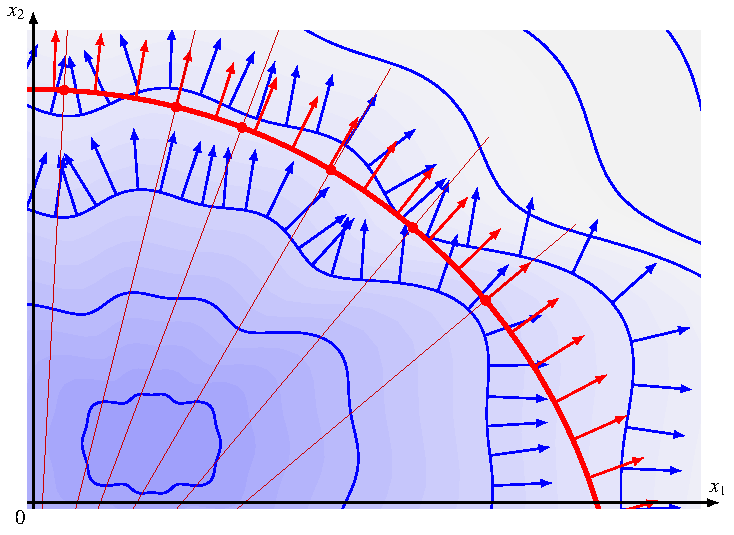
\includegraphics{chapters/010-fuvar/images/nebenbedingung.pdf}
\caption{Extremalproblem für eine Funktion ${\color{blue}f(x,y)}$
(dargestellt durch
die {\color{blue}blauen} Niveaulinien) unter einer Nebenbedingung
${\color{darkred}g(x,y)=c}$, was der Vorgabe einer Kurve
({\color{darkred}rot}), auf der das Extremum gefunden werden muss,
entspricht.
Im Extremum sind die Normalen auf den Niveaulinien $\grad f$
parallel zur Normalen $\grad g$ auf der Nebenbedingungskurve.
\label{buch:fuvar:nebenbedingung:fig:nebenbedingung}}
\end{figure}
